% Options for packages loaded elsewhere
\PassOptionsToPackage{unicode}{hyperref}
\PassOptionsToPackage{hyphens}{url}
%
\documentclass[
  7pt,
]{article}
\usepackage{amsmath,amssymb}
\usepackage{lmodern}
\usepackage{ifxetex,ifluatex}
\ifnum 0\ifxetex 1\fi\ifluatex 1\fi=0 % if pdftex
  \usepackage[T1]{fontenc}
  \usepackage[utf8]{inputenc}
  \usepackage{textcomp} % provide euro and other symbols
\else % if luatex or xetex
  \usepackage{unicode-math}
  \defaultfontfeatures{Scale=MatchLowercase}
  \defaultfontfeatures[\rmfamily]{Ligatures=TeX,Scale=1}
\fi
% Use upquote if available, for straight quotes in verbatim environments
\IfFileExists{upquote.sty}{\usepackage{upquote}}{}
\IfFileExists{microtype.sty}{% use microtype if available
  \usepackage[]{microtype}
  \UseMicrotypeSet[protrusion]{basicmath} % disable protrusion for tt fonts
}{}
\makeatletter
\@ifundefined{KOMAClassName}{% if non-KOMA class
  \IfFileExists{parskip.sty}{%
    \usepackage{parskip}
  }{% else
    \setlength{\parindent}{0pt}
    \setlength{\parskip}{6pt plus 2pt minus 1pt}}
}{% if KOMA class
  \KOMAoptions{parskip=half}}
\makeatother
\usepackage{xcolor}
\IfFileExists{xurl.sty}{\usepackage{xurl}}{} % add URL line breaks if available
\IfFileExists{bookmark.sty}{\usepackage{bookmark}}{\usepackage{hyperref}}
\hypersetup{
  pdftitle={Coding Tasks on dplyr, tidyr and ggplot2 - 17th May 2021},
  pdfauthor={Mario Keller},
  hidelinks,
  pdfcreator={LaTeX via pandoc}}
\urlstyle{same} % disable monospaced font for URLs
\usepackage[left=1cm,right=1cm,top=1.5cm,bottom=1.5cm]{geometry}
\usepackage{color}
\usepackage{fancyvrb}
\newcommand{\VerbBar}{|}
\newcommand{\VERB}{\Verb[commandchars=\\\{\}]}
\DefineVerbatimEnvironment{Highlighting}{Verbatim}{commandchars=\\\{\}}
% Add ',fontsize=\small' for more characters per line
\usepackage{framed}
\definecolor{shadecolor}{RGB}{248,248,248}
\newenvironment{Shaded}{\begin{snugshade}}{\end{snugshade}}
\newcommand{\AlertTok}[1]{\textcolor[rgb]{0.94,0.16,0.16}{#1}}
\newcommand{\AnnotationTok}[1]{\textcolor[rgb]{0.56,0.35,0.01}{\textbf{\textit{#1}}}}
\newcommand{\AttributeTok}[1]{\textcolor[rgb]{0.77,0.63,0.00}{#1}}
\newcommand{\BaseNTok}[1]{\textcolor[rgb]{0.00,0.00,0.81}{#1}}
\newcommand{\BuiltInTok}[1]{#1}
\newcommand{\CharTok}[1]{\textcolor[rgb]{0.31,0.60,0.02}{#1}}
\newcommand{\CommentTok}[1]{\textcolor[rgb]{0.56,0.35,0.01}{\textit{#1}}}
\newcommand{\CommentVarTok}[1]{\textcolor[rgb]{0.56,0.35,0.01}{\textbf{\textit{#1}}}}
\newcommand{\ConstantTok}[1]{\textcolor[rgb]{0.00,0.00,0.00}{#1}}
\newcommand{\ControlFlowTok}[1]{\textcolor[rgb]{0.13,0.29,0.53}{\textbf{#1}}}
\newcommand{\DataTypeTok}[1]{\textcolor[rgb]{0.13,0.29,0.53}{#1}}
\newcommand{\DecValTok}[1]{\textcolor[rgb]{0.00,0.00,0.81}{#1}}
\newcommand{\DocumentationTok}[1]{\textcolor[rgb]{0.56,0.35,0.01}{\textbf{\textit{#1}}}}
\newcommand{\ErrorTok}[1]{\textcolor[rgb]{0.64,0.00,0.00}{\textbf{#1}}}
\newcommand{\ExtensionTok}[1]{#1}
\newcommand{\FloatTok}[1]{\textcolor[rgb]{0.00,0.00,0.81}{#1}}
\newcommand{\FunctionTok}[1]{\textcolor[rgb]{0.00,0.00,0.00}{#1}}
\newcommand{\ImportTok}[1]{#1}
\newcommand{\InformationTok}[1]{\textcolor[rgb]{0.56,0.35,0.01}{\textbf{\textit{#1}}}}
\newcommand{\KeywordTok}[1]{\textcolor[rgb]{0.13,0.29,0.53}{\textbf{#1}}}
\newcommand{\NormalTok}[1]{#1}
\newcommand{\OperatorTok}[1]{\textcolor[rgb]{0.81,0.36,0.00}{\textbf{#1}}}
\newcommand{\OtherTok}[1]{\textcolor[rgb]{0.56,0.35,0.01}{#1}}
\newcommand{\PreprocessorTok}[1]{\textcolor[rgb]{0.56,0.35,0.01}{\textit{#1}}}
\newcommand{\RegionMarkerTok}[1]{#1}
\newcommand{\SpecialCharTok}[1]{\textcolor[rgb]{0.00,0.00,0.00}{#1}}
\newcommand{\SpecialStringTok}[1]{\textcolor[rgb]{0.31,0.60,0.02}{#1}}
\newcommand{\StringTok}[1]{\textcolor[rgb]{0.31,0.60,0.02}{#1}}
\newcommand{\VariableTok}[1]{\textcolor[rgb]{0.00,0.00,0.00}{#1}}
\newcommand{\VerbatimStringTok}[1]{\textcolor[rgb]{0.31,0.60,0.02}{#1}}
\newcommand{\WarningTok}[1]{\textcolor[rgb]{0.56,0.35,0.01}{\textbf{\textit{#1}}}}
\usepackage{graphicx}
\makeatletter
\def\maxwidth{\ifdim\Gin@nat@width>\linewidth\linewidth\else\Gin@nat@width\fi}
\def\maxheight{\ifdim\Gin@nat@height>\textheight\textheight\else\Gin@nat@height\fi}
\makeatother
% Scale images if necessary, so that they will not overflow the page
% margins by default, and it is still possible to overwrite the defaults
% using explicit options in \includegraphics[width, height, ...]{}
\setkeys{Gin}{width=\maxwidth,height=\maxheight,keepaspectratio}
% Set default figure placement to htbp
\makeatletter
\def\fps@figure{htbp}
\makeatother
\setlength{\emergencystretch}{3em} % prevent overfull lines
\providecommand{\tightlist}{%
  \setlength{\itemsep}{0pt}\setlength{\parskip}{0pt}}
\setcounter{secnumdepth}{5}
\makeatletter\renewcommand*{\fps@figure}{h}\makeatother
\usepackage{placeins}
\ifluatex
  \usepackage{selnolig}  % disable illegal ligatures
\fi

\title{Coding Tasks on dplyr, tidyr and ggplot2 - 17th May 2021}
\author{Mario Keller}
\date{May 10, 2021}

\begin{document}
\maketitle

{
\setcounter{tocdepth}{3}
\tableofcontents
}
\pagebreak

\hypertarget{introduction}{%
\section{Introduction}\label{introduction}}

A good bioinformatician not only produces huge amounts of data, but is
also able to cleanse and adjust these in order to then produce plots
that are ready for publication. In today's coding task we will have a
look on 3 R packges that are useful for the mentioned tasks.

The first of these packages is
\href{https://dplyr.tidyverse.org/}{dplyr}, which offers a grammar for
data manipulation. The second package is
\href{https://tidyr.tidyverse.org/}{tidyr}, which helps you to clean up
your data. The third package is
\href{https://ggplot2.tidyverse.org/}{ggplot2}, which helps your to
create good looking graphics that can be adjusted down to the smallest
detail.

We will not fully explore the complete functionality of these packages
but have a look on the most important functions. For further details
check out the websites of the packages that are placed as a hyperlink in
the package names above.

\hypertarget{required-libraries}{%
\section{Required libraries}\label{required-libraries}}

The following libraries and data are required in today's coding tasks.

\begin{Shaded}
\begin{Highlighting}[]
\FunctionTok{library}\NormalTok{(dplyr)}
\FunctionTok{library}\NormalTok{(tidyr)}
\FunctionTok{library}\NormalTok{(ggplot2)}
\FunctionTok{library}\NormalTok{(gridExtra)}

\CommentTok{\#Adjust the path for your system}
\NormalTok{TPM.df }\OtherTok{\textless{}{-}}\FunctionTok{readRDS}\NormalTok{(}\StringTok{"data/TPM.df.rds"}\NormalTok{) }
\end{Highlighting}
\end{Shaded}

\hypertarget{dplyr}{%
\section{dplyr}\label{dplyr}}

One of the most important aspects about the dplyr packages is the
so-called pipe operator \textbf{\%\textgreater\%}. This operator allows
you to chain together sets of operations in a very intuitive fashion.
Here is one example where we create a data frame, for which we calculate
the mean for each row and afterwards the mean of the computed row means:

\begin{Shaded}
\begin{Highlighting}[]
\CommentTok{\#With nested parentheses.}
\FunctionTok{mean}\NormalTok{(}\FunctionTok{rowMeans}\NormalTok{(}\FunctionTok{data.frame}\NormalTok{(}\AttributeTok{x=}\DecValTok{1}\SpecialCharTok{:}\DecValTok{10}\NormalTok{, }\AttributeTok{y=}\DecValTok{1}\SpecialCharTok{:}\DecValTok{10}\NormalTok{)))}
\end{Highlighting}
\end{Shaded}

\begin{verbatim}
## [1] 5.5
\end{verbatim}

\begin{Shaded}
\begin{Highlighting}[]
\CommentTok{\#With \%\textgreater{}\%}
\FunctionTok{data.frame}\NormalTok{(}\AttributeTok{x=}\DecValTok{1}\SpecialCharTok{:}\DecValTok{10}\NormalTok{, }\AttributeTok{y=}\DecValTok{1}\SpecialCharTok{:}\DecValTok{10}\NormalTok{) }\SpecialCharTok{\%\textgreater{}\%}\NormalTok{ rowMeans }\SpecialCharTok{\%\textgreater{}\%}\NormalTok{ mean}
\end{Highlighting}
\end{Shaded}

\begin{verbatim}
## [1] 5.5
\end{verbatim}

As you can see, using the \%\textgreater\% operator is much more
intuitive than using nested parentheses.

In addition the dplyr package offers additional functions that help you
to filter your data, add new columns, adjust existing columns and
arrange your data frames.

\hypertarget{task1---level-beginner}{%
\subsection{Task1 - Level: Beginner}\label{task1---level-beginner}}

Use the function filter() to filter for patients, whose Gene1 TPM values
in brain and liver are \textgreater{} 150 and use afterwards arrange()
to order the patients in descending order by their Gene1 Brain TPM
value. Use the \%\textgreater\% operator and continue with the filtered
data frame.

Hint: You should end up with 731 patients.

\hypertarget{task2---level-advanced}{%
\subsection{Task2 - Level: Advanced}\label{task2---level-advanced}}

Create a new column called sumVar which contains the sum of
Gene1\_Brain, Gene2\_Brain, Gene1\_Liver and Gene2\_Liver for each
patient. Afterwards filter for patients where sumVar \textgreater{} 500
and subsequently remove the sumVar column with select(). Helpful
functions are mutate(), rowwise() and c\_across(). Use the
\%\textgreater\% operator.

Hint: Check out the example in ?c\_across. You should end up with 679
patients. The data frame is now a tibble, which is just an advanced data
frame.

\hypertarget{tidyr}{%
\section{tidyr}\label{tidyr}}

If you did not solve Task2 load the data.frame stored in
``TPM.df.tidyr.rds'' and continue with this data frame.

The tidyr package offers different functions for cleaning up your data
frames such as changing them from a wide to long format nad vice versa.

\hypertarget{task3---level-beginner}{%
\subsection{Task3 - Level: Beginner}\label{task3---level-beginner}}

We will now mimic a scenario where for one of the patients the
Gene1\_Brain value is missing. Enter for the patient in row 3 an NA in
the Gene1\_Brain column (e.g.~TPM.df{[}3,2{]} \textless- NA or
TPM.df\$Gene1\_Brain{[}3{]} \textless- NA). Use replace\_na() to replace
the NA in the Gene1\_Brain column with 361.0915.

Hint: replace() needs a list that contains the replacement values for
each column.

\hypertarget{task4---level-advanced}{%
\subsection{Task4 - Level: Advanced}\label{task4---level-advanced}}

At the moment we have data frame in a wide format. However, we want it
to be in a long format. Use pivot\_longer() to produce a data frame
where each combination of patient, gene and tissue is a single row.

Hint: You can split the names of the columns 2 to 5 by "\_" and use
``Gene'' and ``Tissue'' as new column names. In addition the values
column could be called ``TPM''.

This is how the data frame should look like:

\begin{verbatim}
## # A tibble: 8 x 4
##   Patien.ID Gene  Tissue   TPM
##   <fct>     <chr> <chr>  <dbl>
## 1 164       Gene1 Brain  394. 
## 2 164       Gene2 Brain   88.1
## 3 164       Gene1 Liver  189. 
## 4 164       Gene2 Liver   82.4
## 5 747       Gene1 Brain  362. 
## 6 747       Gene2 Brain   71.2
## 7 747       Gene1 Liver  195. 
## 8 747       Gene2 Liver   91.9
\end{verbatim}

\hypertarget{task5---level-advanced}{%
\subsection{Task5 - Level: Advanced}\label{task5---level-advanced}}

We can also go from a long format to a wide format. Use pivot\_wider()
to make two columns out of the ``Gene'' column.

Hint: The parameters ``names\_from'' and ``values\_from'' are helpful.

This is how the data frame should look like:

\begin{verbatim}
## # A tibble: 6 x 4
##   Patien.ID Tissue Gene1 Gene2
##   <fct>     <chr>  <dbl> <dbl>
## 1 164       Brain   394.  88.1
## 2 164       Liver   189.  82.4
## 3 747       Brain   362.  71.2
## 4 747       Liver   195.  91.9
## 5 842       Brain   361.  73.7
## 6 842       Liver   170.  76.4
\end{verbatim}

\hypertarget{ggplot2}{%
\section{ggplot2}\label{ggplot2}}

If you did not solve Task5 load the data.frame stored in
``TPM.df.ggplot2.rds'' and continue with this data frame.

The ggplot2 package offers a modular structure that allows you to
generate plots layer by layer. The most important function is ggplot()
that initializes a ggplot object in which we declare the input data
frame and set the plot aesthetics. The aesthetics are defined within
ggplot() by using aes(). Aesthetics tell ggplot which columns contain
the values on the x- and y-axis or which column should be used as a
color or fill. After we have initialized a ggplot object with ggplot()
we can add layers with the plus sign (+). Here are some examples of
layers:

\begin{itemize}
\tightlist
\item
  geom\_point() for scatter plots
\item
  geom\_line() for line plots
\item
  geom\_col() for bar charts
\item
  geom\_histogram() for histograms
\item
  geom\_density() for density plots
\end{itemize}

In addition there are different functions that can be used to adjust the
x- and y-axis, to set labels or to set a user-defined color-scale.

Here is a simple example that shows how to create a scatter plot and to
color the points by a certain column in the data.frame

\begin{Shaded}
\begin{Highlighting}[]
\CommentTok{\#Create the data frame}
\FunctionTok{data.frame}\NormalTok{(}\AttributeTok{column1=}\DecValTok{1}\SpecialCharTok{:}\DecValTok{10}\NormalTok{, }\AttributeTok{column2=}\DecValTok{1}\SpecialCharTok{:}\DecValTok{10}\NormalTok{, }\AttributeTok{cat=}\FunctionTok{factor}\NormalTok{(}\FunctionTok{rep}\NormalTok{(}\FunctionTok{c}\NormalTok{(}\StringTok{"a"}\NormalTok{,}\StringTok{"b"}\NormalTok{),}\DecValTok{5}\NormalTok{), }\AttributeTok{levels=}\FunctionTok{c}\NormalTok{(}\StringTok{"a"}\NormalTok{, }\StringTok{"b"}\NormalTok{))) }\SpecialCharTok{\%\textgreater{}\%} 
  \CommentTok{\#Initialize the ggplot object}
  \FunctionTok{ggplot}\NormalTok{(., }\FunctionTok{aes}\NormalTok{(}\AttributeTok{x=}\NormalTok{column1, }\AttributeTok{y=}\NormalTok{column2, }\AttributeTok{color=}\NormalTok{cat)) }\SpecialCharTok{+}
  \CommentTok{\#Add a layer with points}
  \FunctionTok{geom\_point}\NormalTok{(}\AttributeTok{size=}\DecValTok{3}\NormalTok{) }\SpecialCharTok{+}
  \CommentTok{\#Add a layer with a line}
  \FunctionTok{geom\_line}\NormalTok{(}\AttributeTok{col=}\StringTok{"black"}\NormalTok{) }\SpecialCharTok{+}
  \CommentTok{\#Re{-}name the axes and set a title}
  \FunctionTok{labs}\NormalTok{(}\AttributeTok{x=}\StringTok{"x{-}axis"}\NormalTok{, }\AttributeTok{y=}\StringTok{"y{-}axis"}\NormalTok{, }\AttributeTok{title=}\StringTok{"My first plot"}\NormalTok{)}
\end{Highlighting}
\end{Shaded}

\begin{center}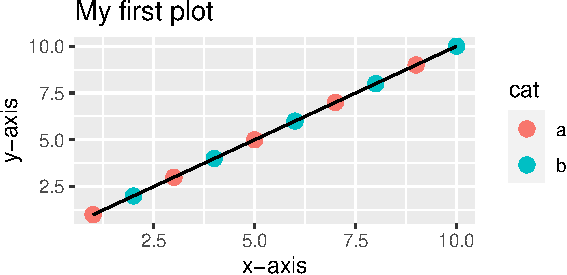
\includegraphics{dplyr_tidyr_ggplot2_files/figure-latex/ggplot_example-1} \end{center}

Once you have internalized the ggplot philosophy it is very easy to
create beautiful plots that nicely represent your results.

\hypertarget{task6---level-beginner}{%
\subsection{Task6 - Level: Beginner}\label{task6---level-beginner}}

We want to make for each of the two tissues a scatter plot to show the
correlation between Gene1 and Gene2. One easy way is to first subset the
data.frame to have a single data frame for each of the tissues, create
the plot and store it in a variable. Subset the data.frame once for the
Brain tissue and once for the Liver tissue and store the two data frames
as Brain.TPM.df and Liver.TPM.df

Hint: The subset() function is very useful.

\pagebreak

\hypertarget{task7---level-beginner}{%
\subsection{Task7 - Level: Beginner}\label{task7---level-beginner}}

Use the two data frames to create two scatter plots using geom\_point()
with Gene1 on the x- and Gene 2 on the y-axis and store them as
Brain.plot and Liver.plot. Afterwards use grid.arrange() from the
gridExtra package to combine the two plots into a single plot
side-by-side.

Hint: x and y are defined in aes(). You can tell grid.arrange whether
you want the plots side by side or on top of each other (check out ncol
and nrow).

\begin{center}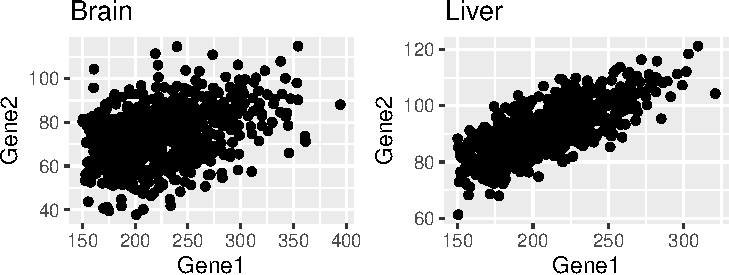
\includegraphics{dplyr_tidyr_ggplot2_files/figure-latex/task7-1} \end{center}

\hypertarget{task8---level-advanced}{%
\subsection{Task8 - Level: Advanced}\label{task8---level-advanced}}

An alternative to the above approach is to use facet\_wrap() from the
ggplot2 package to automatically create subplots. Use the TPM.df with
facet\_wrap() to create two subplots based on the Tissue column. In
addition, color the the points by Tissue.

\begin{center}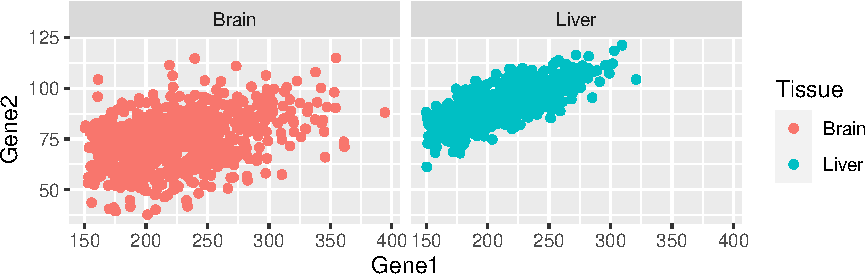
\includegraphics{dplyr_tidyr_ggplot2_files/figure-latex/task8-1} \end{center}

\hypertarget{task9---level-advanced}{%
\subsection{Task9 - Level: Advanced}\label{task9---level-advanced}}

As you can see the two plots share the same x- and y-axis. Try to set
for each plot individual axes.

Hint: Check out ?facet\_wrap to find out how you can create for each
plot individual x- and y-axes.

\begin{center}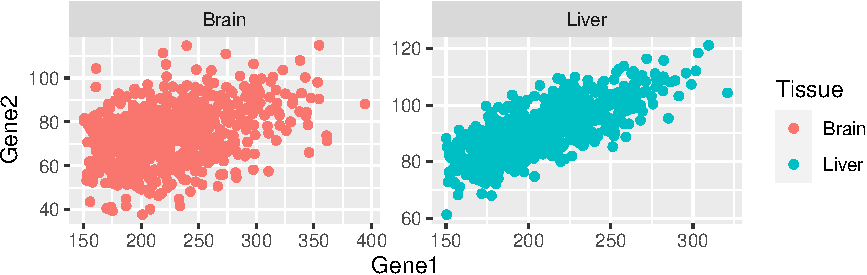
\includegraphics{dplyr_tidyr_ggplot2_files/figure-latex/task9-1} \end{center}

\hypertarget{task10---level-advanced}{%
\subsection{Task10 - Level: Advanced}\label{task10---level-advanced}}

When we try to look at correlations a regression line is often helpful.
Use geom\_smooth() to add a black regression line as a new layer.

Hint: Check out ?geom\_smooth and look for the correct ``method''. lm
could be useful.

\begin{center}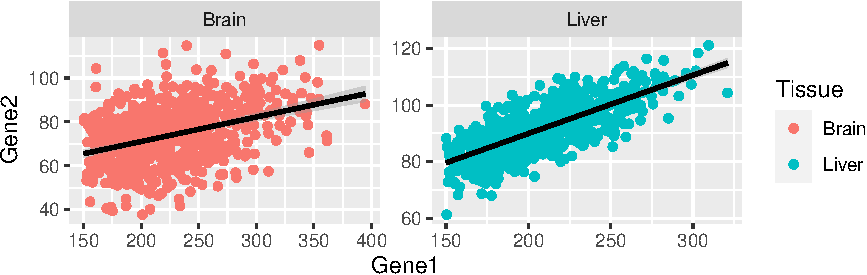
\includegraphics{dplyr_tidyr_ggplot2_files/figure-latex/task10-1} \end{center}

\end{document}
